\noindent

\includegraphics[height=1.25cm]{images/pictograms/benchmark}

\includegraphics[height=1.25cm]{images/pictograms/under_construction}

\includegraphics[height=1.25cm]{images/pictograms/FEM}

\includegraphics[height=1.25cm]{images/pictograms/paraview}

%%%%%%%%%%%%%%%%%%%%%%%%%%%%%%%%%%%%%%%%%%%%%%%%%%%%%%%%%%%%%%%%%%%%%%%%%%%%%%%%%%%%%%%%%%%%%%%%%%%

\begin{flushright} {\tiny {\color{gray} python\_codes/fieldstone\_133/text.tex}} \end{flushright}

%\lstinputlisting[language=bash,basicstyle=\small]{python_codes/template_keywords.key}

\par\noindent\rule{\textwidth}{0.4pt}

\begin{center}
\inpython
{\small Code: \url{https://github.com/cedrict/fieldstone/tree/master/python_codes/fieldstone_133}}
\end{center}

\par\noindent\rule{\textwidth}{0.4pt}
%%%%%%%%%%%%%%%%%%%%%%%%%%%%%%%%%%%%%%%%%%%%%%%%%%%%%%%%%%%%%%%%%%%%%%%%%%%%%%%%%%%%%%%%%%%%

The benchmark is described fully in Section~\ref{MMM-ss:anconv}. 
The following results have been obtained with $k=4$.
Taylor-Hood $Q_2\times Q_1$ elements are used with an isoparametric mapping. 
This \stone is based on \stone~21 (please refer to this one first 
before reading any further).

The idea here is to test the Double Jacobian algorithm presented in \textcite{moth20} (2020)
as thoroughly described and worked out in Section~\ref{MMM-ss:doublejac}.

In the code this can be toggled on/off by means of the {\python DJ} boolean.
Also, the internal numbering of nodes has been completely reworked with regards to 
the one used in \stone~21 to match best with the theory notations.

The node layout is as follows (in this case nelr=1, nelt=4, so four $Q_2$ elements:

\begin{center}
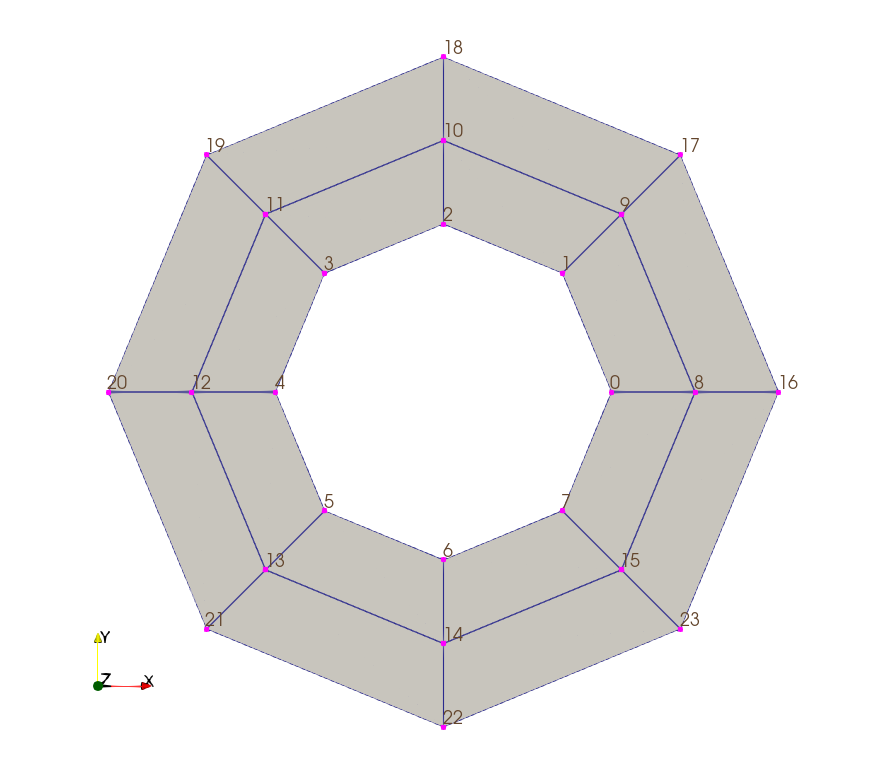
\includegraphics[width=8cm]{python_codes/fieldstone_133/images/nodes}
\end{center}
with
\begin{verbatim}
nelr= 1
nelt= 4
nel= 4
NfemV= 48
NfemP= 8
0 | [ 0 16 18  2  8 17 10  1  9]
1 | [ 2 18 20  4 10 19 12  3 11]
2 | [ 4 20 22  6 12 21 14  5 13]
3 | [ 6 22 16  0 14 23  8  7 15]
\end{verbatim}

As mentioned in the paper, one of the drawbacks of the double Jacobian 
is the fact that the terms to be integrated are no more polynomials, so
that it is not straightforward to determine the necessary number of 
quadrature points. I have introduced the {\python nqperdim} parameter
which allows to control the number of quadrature points per dimension.
We will be testing 3,4,5,6. 

%------------------------------------------------------------------
\section*{Results}

%-------------------------
\subsection*{benchmark 1}

Using isoparametric mapping, we obtain the following results.
As documented in \stone~21, we recover a 3rd order convergence for the velocity error
and a 2nd order convergence for the pressure error.

\begin{center}
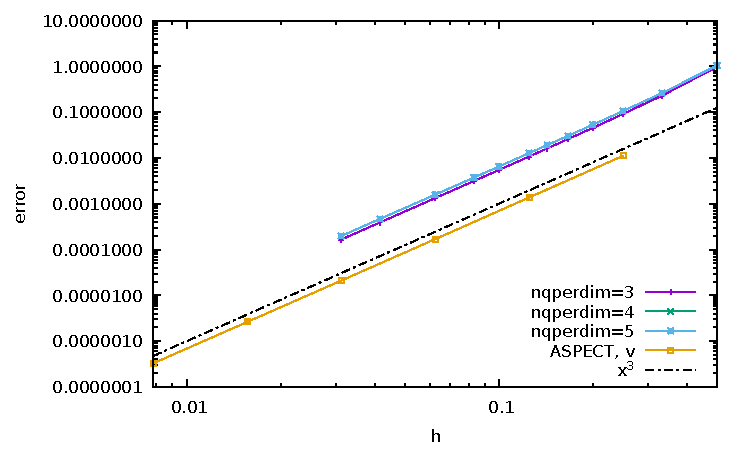
\includegraphics[width=5.7cm]{python_codes/fieldstone_133/results/bench1/errors_v.pdf}
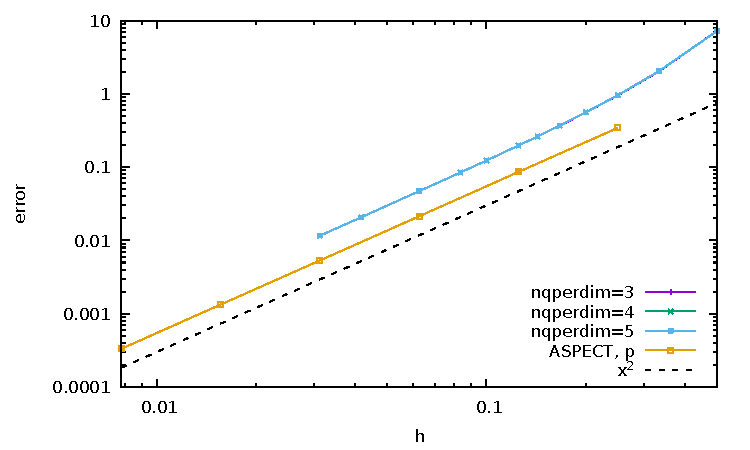
\includegraphics[width=5.7cm]{python_codes/fieldstone_133/results/bench1/errors_p.pdf}\\
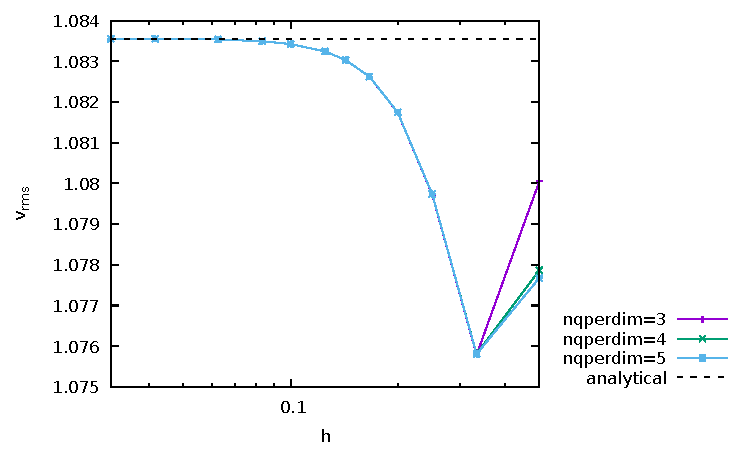
\includegraphics[width=5.7cm]{python_codes/fieldstone_133/results/bench1/vrms.pdf}
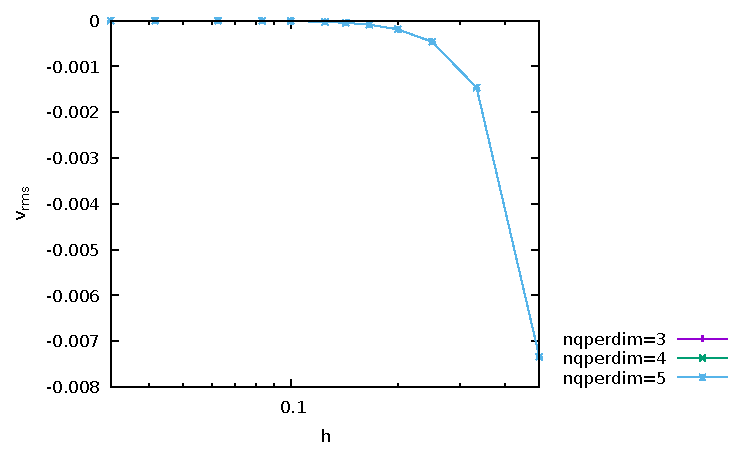
\includegraphics[width=5.7cm]{python_codes/fieldstone_133/results/bench1/area.pdf}
\end{center}

Now switching to DJ:

\begin{center}
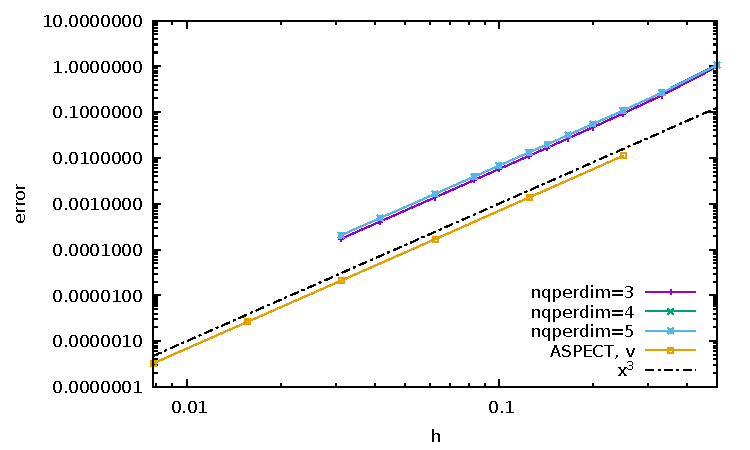
\includegraphics[width=5.7cm]{python_codes/fieldstone_133/results/bench1/DJ/errors_v.pdf}
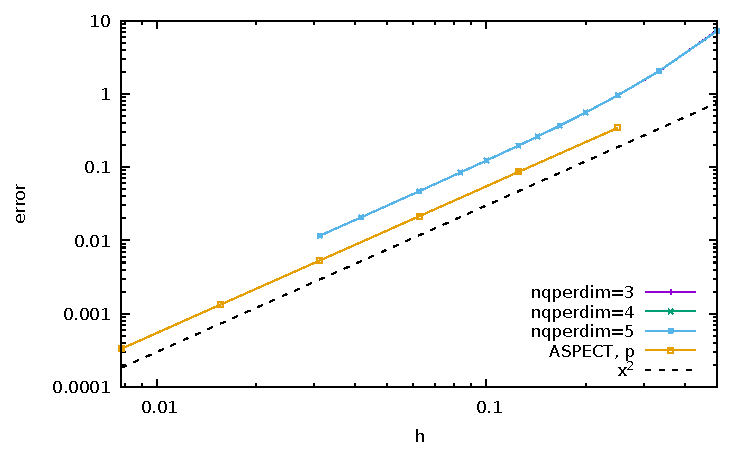
\includegraphics[width=5.7cm]{python_codes/fieldstone_133/results/bench1/DJ/errors_p.pdf}\\
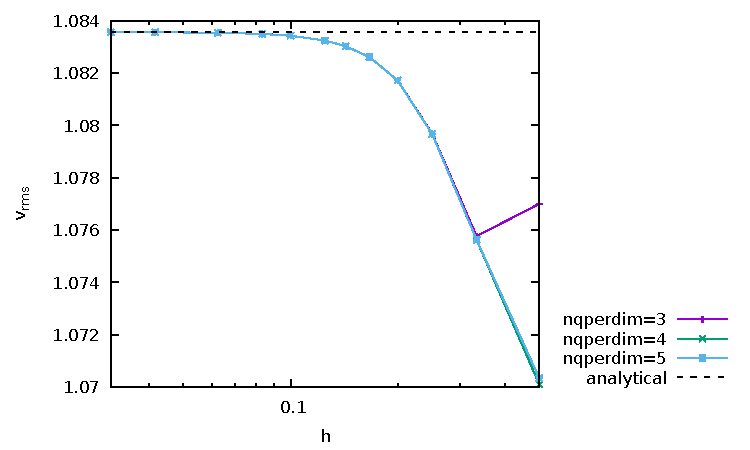
\includegraphics[width=5.7cm]{python_codes/fieldstone_133/results/bench1/DJ/vrms.pdf}
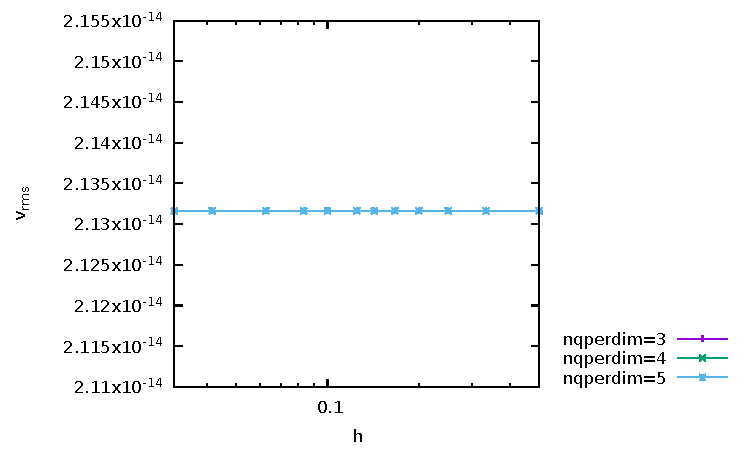
\includegraphics[width=5.7cm]{python_codes/fieldstone_133/results/bench1/DJ/area.pdf}
\end{center}

These results are somewhat disappointing.

%-------------------------
\subsection*{benchmark 2}

Let us now turn to the aquarium benchmark. Gravity is 1, density is $10^6$ and no-slip
boundary conditions are imposed. The solution is a zero velocity and a lithostatic pressure.

\begin{center}
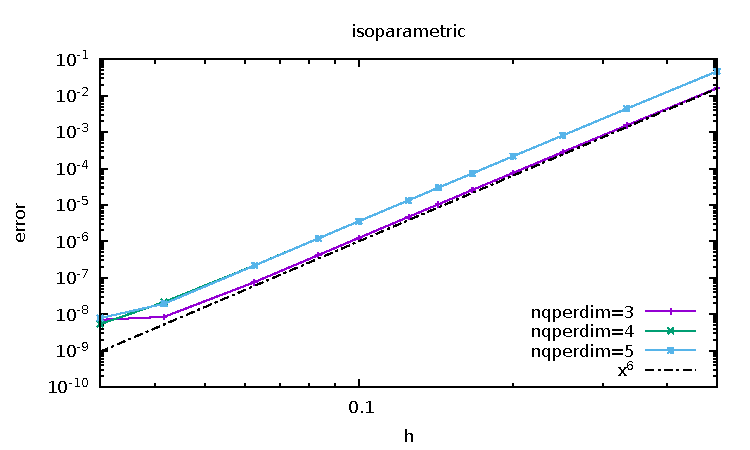
\includegraphics[width=7cm]{python_codes/fieldstone_133/results/bench2/errors_v.pdf}
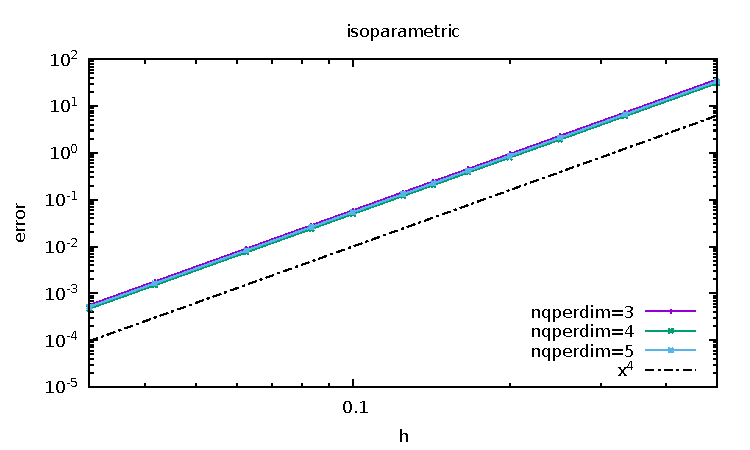
\includegraphics[width=7cm]{python_codes/fieldstone_133/results/bench2/errors_p.pdf}\\
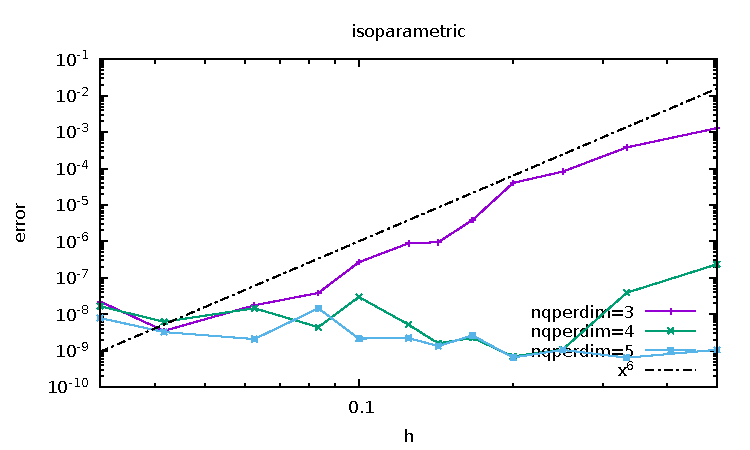
\includegraphics[width=7cm]{python_codes/fieldstone_133/results/bench2/DJ/errors_v.pdf}
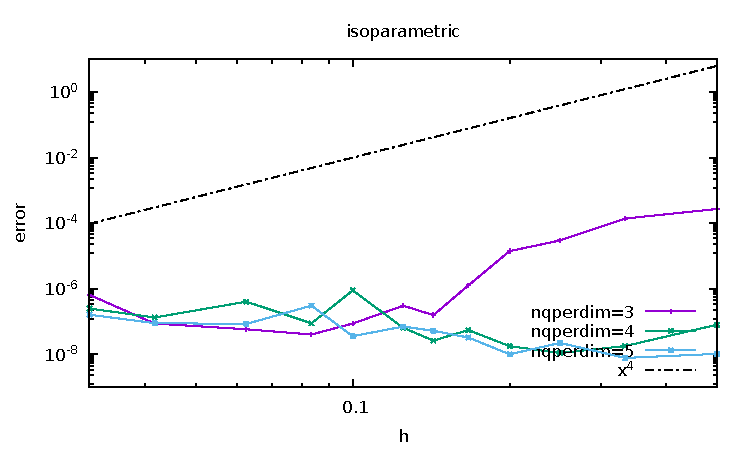
\includegraphics[width=7cm]{python_codes/fieldstone_133/results/bench2/DJ/errors_p.pdf}
\end{center}


\newpage
%-------------------------
\subsection*{benchmark 3}

Same idea as benchmark 2, but now it is Earth-like: $R_1=2890~\si{\km}$, $R_2=6370~\si{\km}$, 
$\rho=4000~\si{\kg\per\cubic\meter}$, $\eta=10^{21}~\si{\pascal\second}$, 
$g=10~\si{\meter\per\square\second}$.

I screwed up! $R_1$ should have been 3480!

\begin{center}
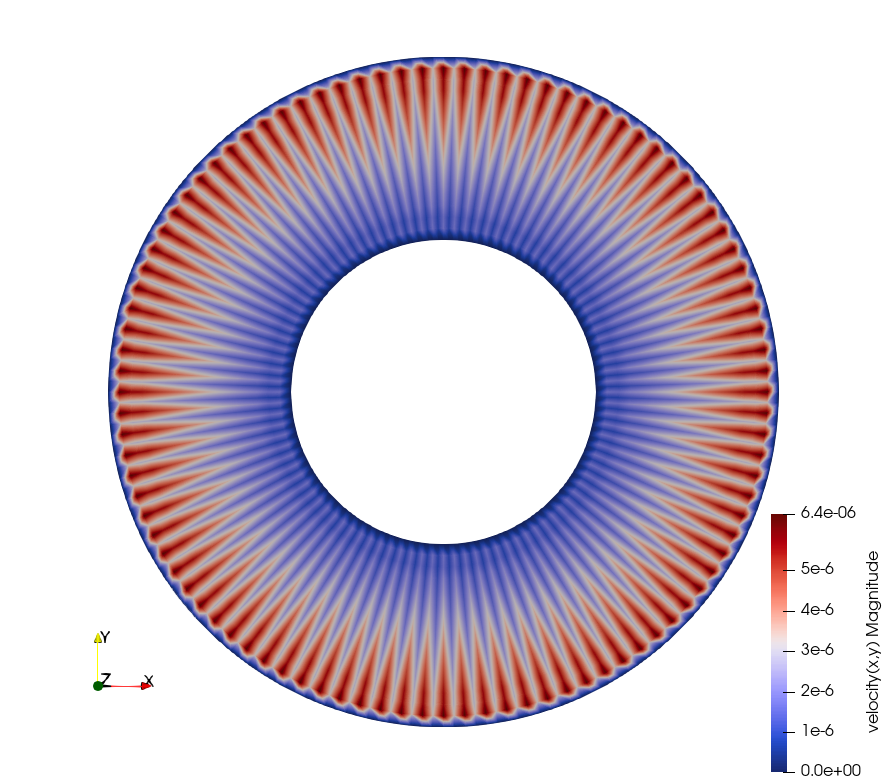
\includegraphics[width=4cm]{python_codes/fieldstone_133/results/bench3/vel}\\
{\captionfont  Velocity field for nelr=8 Q2Q1 elements, isoparametric mapping.}
\end{center}

\begin{center}
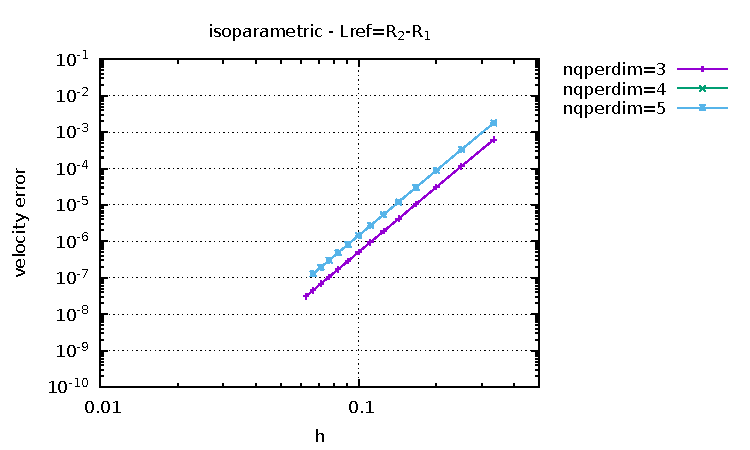
\includegraphics[width=7cm]{python_codes/fieldstone_133/results/bench3/ISO_Lref_R21/errors_v.pdf}
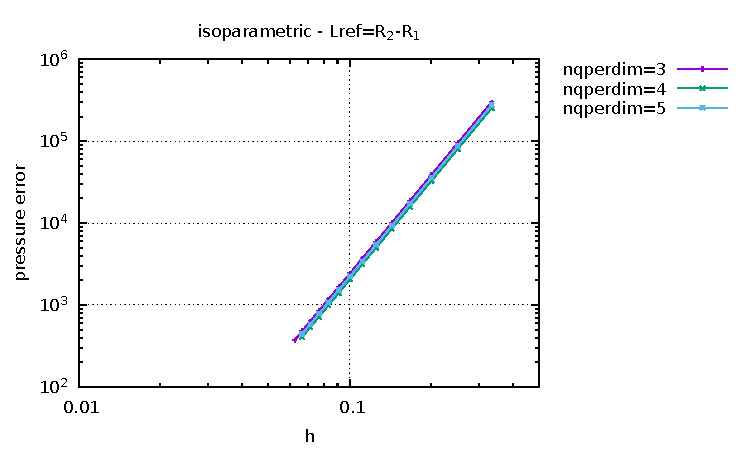
\includegraphics[width=7cm]{python_codes/fieldstone_133/results/bench3/ISO_Lref_R21/errors_p.pdf}\\
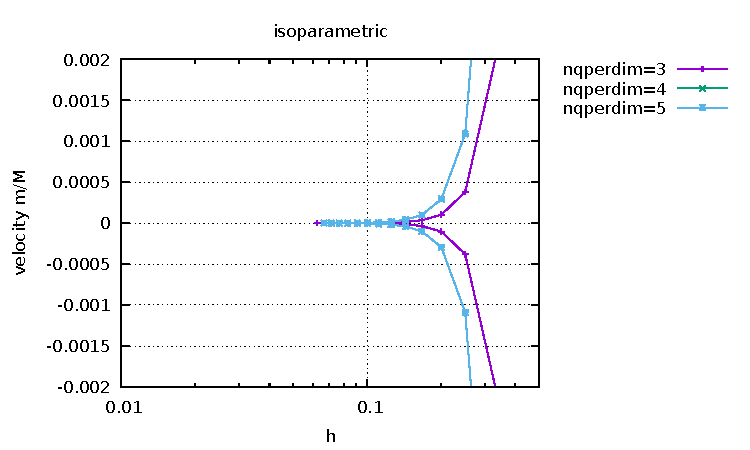
\includegraphics[width=7cm]{python_codes/fieldstone_133/results/bench3/ISO_Lref_R21/vel_stats.pdf}
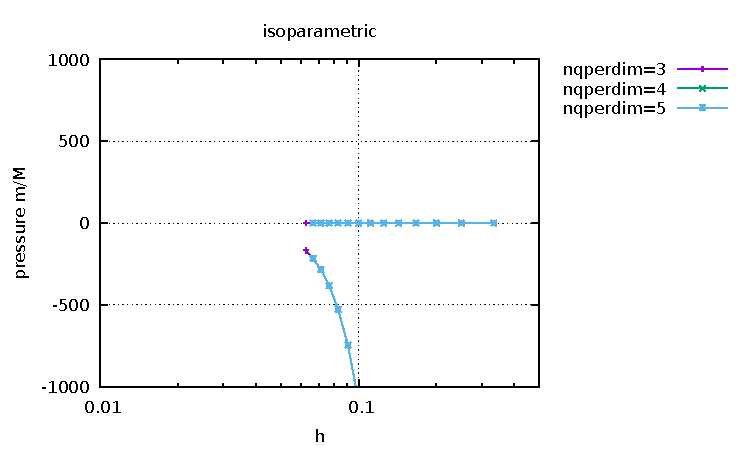
\includegraphics[width=7cm]{python_codes/fieldstone_133/results/bench3/ISO_Lref_R21/press_stats.pdf}\\
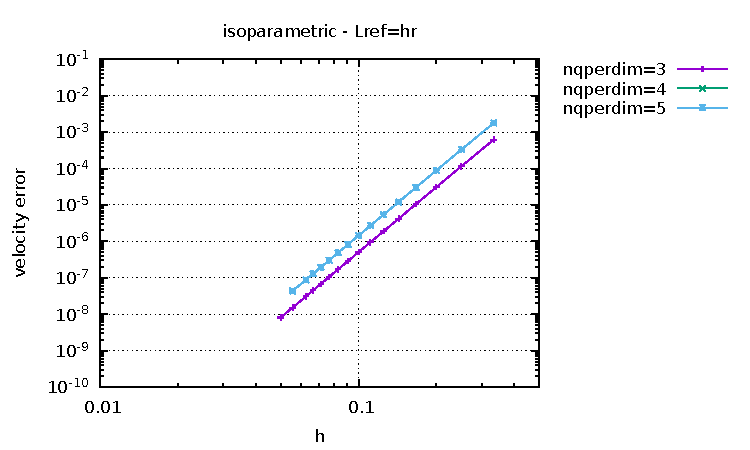
\includegraphics[width=7cm]{python_codes/fieldstone_133/results/bench3/ISO_Lref_hr/errors_v.pdf}
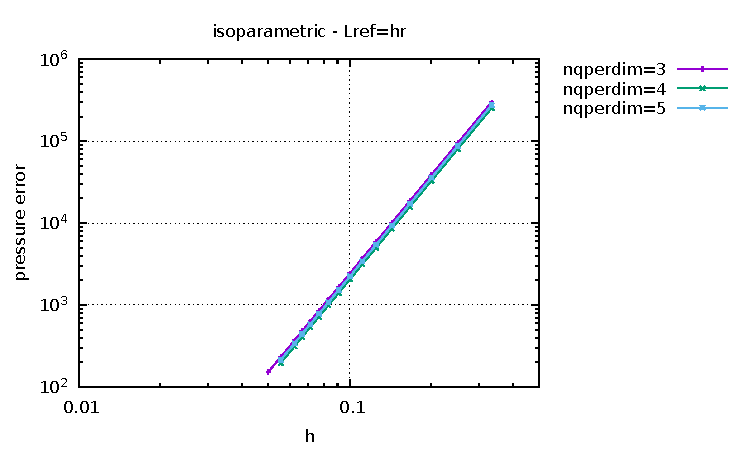
\includegraphics[width=7cm]{python_codes/fieldstone_133/results/bench3/ISO_Lref_hr/errors_p.pdf}\\
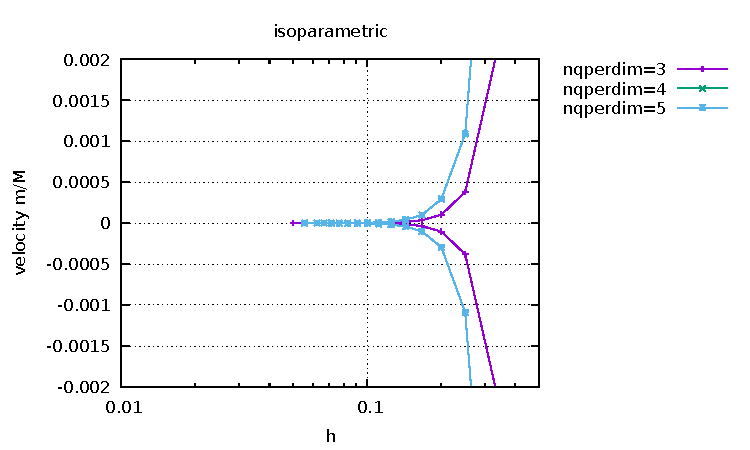
\includegraphics[width=7cm]{python_codes/fieldstone_133/results/bench3/ISO_Lref_hr/vel_stats.pdf}
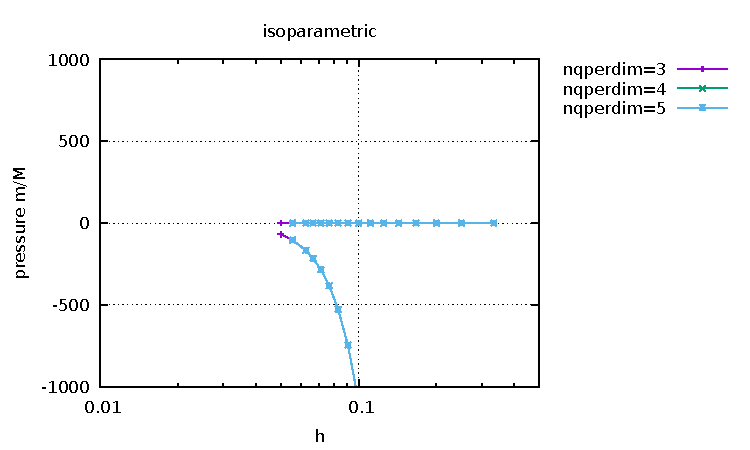
\includegraphics[width=7cm]{python_codes/fieldstone_133/results/bench3/ISO_Lref_hr/press_stats.pdf}\\
{\captionfont Velocities in cm/year.}
\end{center}

Conclusions:

\begin{center}
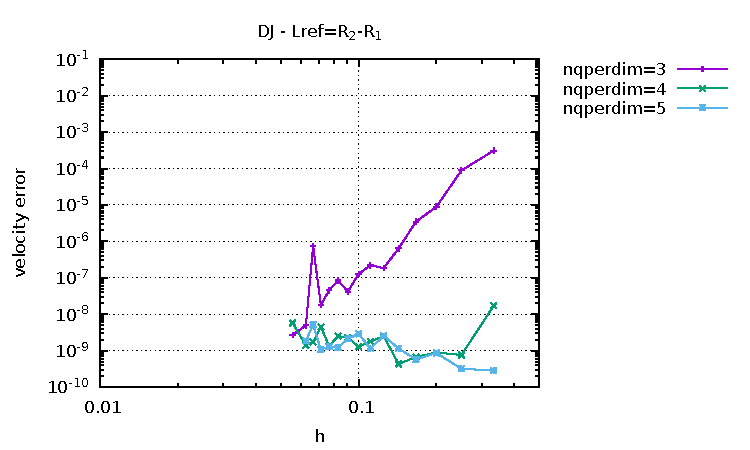
\includegraphics[width=7cm]{python_codes/fieldstone_133/results/bench3/DJ_Lref_R21/errors_v.pdf}
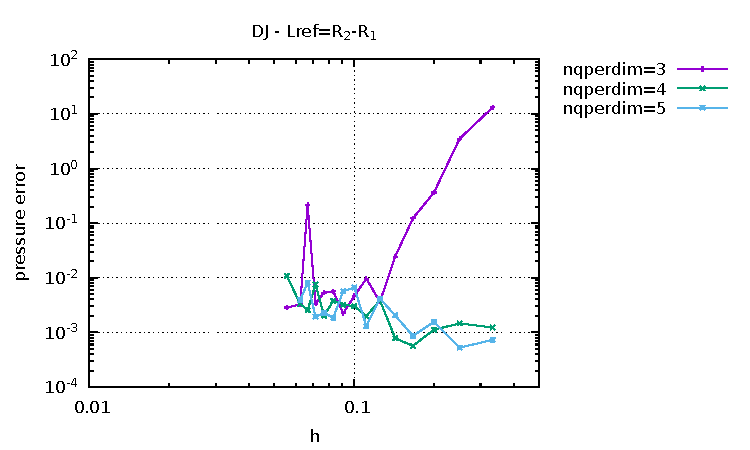
\includegraphics[width=7cm]{python_codes/fieldstone_133/results/bench3/DJ_Lref_R21/errors_p.pdf}\\
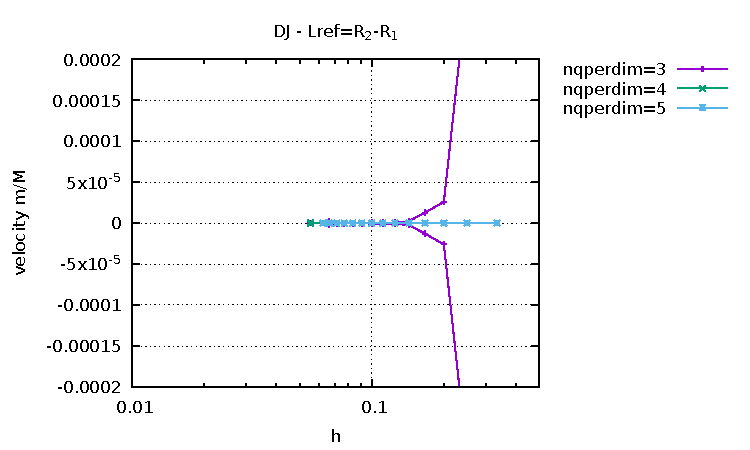
\includegraphics[width=7cm]{python_codes/fieldstone_133/results/bench3/DJ_Lref_R21/vel_stats.pdf}
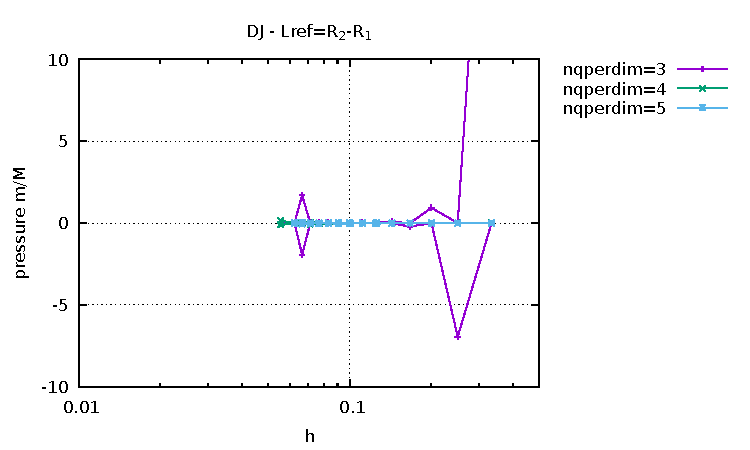
\includegraphics[width=7cm]{python_codes/fieldstone_133/results/bench3/DJ_Lref_R21/press_stats.pdf}\\
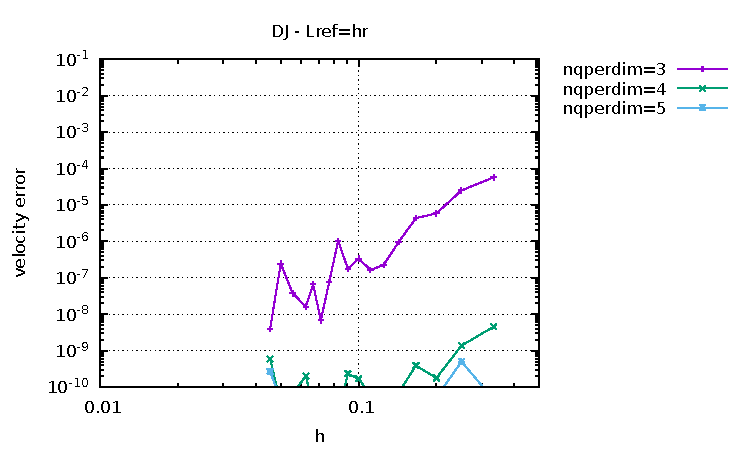
\includegraphics[width=7cm]{python_codes/fieldstone_133/results/bench3/DJ_Lref_hr/errors_v.pdf}
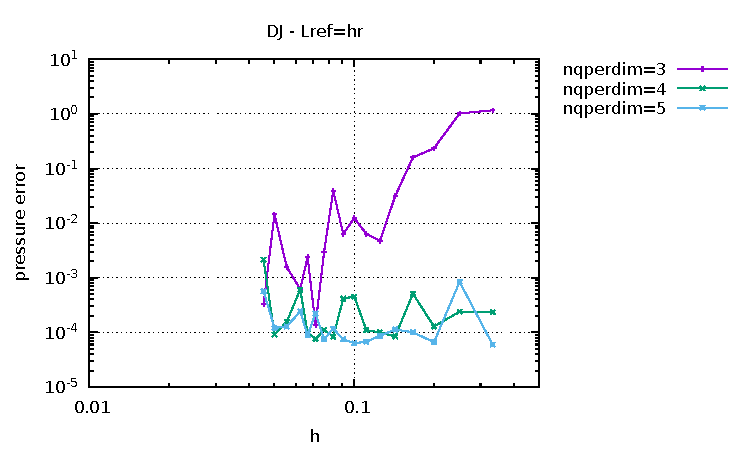
\includegraphics[width=7cm]{python_codes/fieldstone_133/results/bench3/DJ_Lref_hr/errors_p.pdf}\\
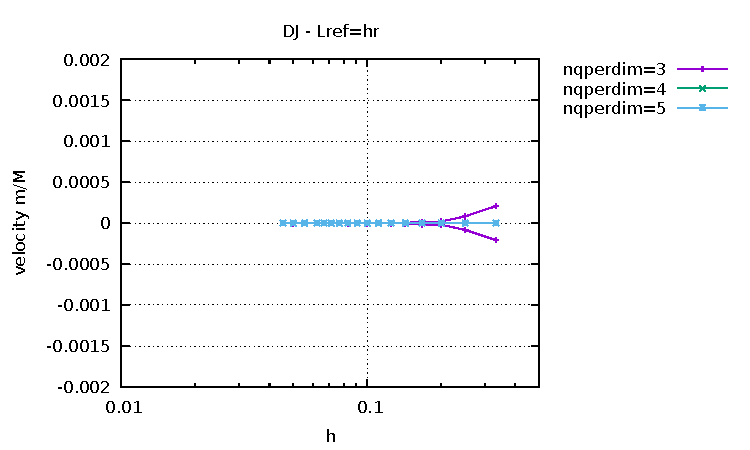
\includegraphics[width=7cm]{python_codes/fieldstone_133/results/bench3/DJ_Lref_hr/vel_stats.pdf}
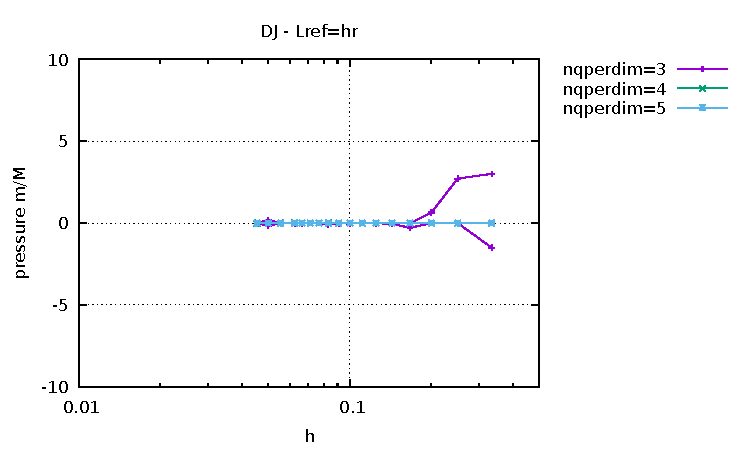
\includegraphics[width=7cm]{python_codes/fieldstone_133/results/bench3/DJ_Lref_hr/press_stats.pdf}\\
{\captionfont Velocities in cm/year.}
\end{center}

Conclusions:

